\section{Validating proof trees}\label{sec:valTree}

After introducing the problem and modeling datalog in Lean, we now describe the algorithm to verify a solution partially. We focus in this section on the soundness by verifying a given proof tree. In the previous section, we introduced the following characterization for valid proof trees:

\begin{lstlisting}
    def isValid(P: program τ) (d: database τ) (t: proofTree τ): 
    Prop :=
    match t with
    | proofTree.node a l => 
    ( ∃(r: rule τ) (g:grounding τ), 
        r ∈ P ∧ 
        ruleGrounding r g = groundRuleFromAtoms a (List.map root l)
        ∧ l.attach.All₂ (fun ⟨x, _h⟩ => isValid P d x)) 
    ∨ (l = [] ∧ d.contains a)
\end{lstlisting}

This is a disjunction so we need procedures to decide for both disjuncts if they are true.
The second disjunct consists of a database check and a check of list emptiness. Both can be done straightforwardly.

The first part is more interesting. Since we use there existential quantifiers, this is not computable and have to implement a function for this. While we can simply iterate over the program to check for the existence of an $r$, the number of groundings might be exponential or even infinite. Instead of using groundings, we want to use some more sophisticated to check this which we introduce next.


\subsection{Substitutions}
    A grounding is a function from variables to constants. This means we always need to specify for every variable a constant that it is mapped to. This was good in the definitions to ensure that we always get a ground atom, but raises problems in the unification case as the following example demonstrates.

    \begin{example}\label{ex:subsGroun}
        Suppose we want to know whether we can unify the list of terms $l_1 = [?x, ?y]$ with the list of constants $l_2= [a,b]$, i.e. we look for a function $f: V \to C$ such that mapping every element of $l_1$ with $f$ yields $l_2$.

        We start by trying to unify $x$ and $a$. If we use groundings, we might use this function $g = x \mapsto a, y \mapsto a, z \mapsto a$.

        Now we want to use this result and match another term $y$ with the constant $b$. The variable $y$ is already mapped to a different constant, but we cannot say whether this is due to a previous matching process or simply because we needed to define a value for every input.         
    \end{example}
    
    One solution might be to use a special constant symbol that we map variables to that are really unmapped for now.
    Instead, we want to use substitutions that were already introduced in \cite{datalogCoq}. A substitution is a partial mapping from variables to constants. We implement this by mapping to an Option of constant.

    \begin{lstlisting}
    def (.\substitution.) (τ: signature):= τ.vars → Option (τ.constants)
    \end{lstlisting}

    This allows us to only specify what is necessary. We call the substitution that maps any variable to none the empty substitution.
    
    If we apply a substitution to a term and this term is a constant, we do not change the term. If the term is a variable and the substitution does not map the variable to none we replace the variable with the result of the substitution.

    \begin{lstlisting}
    def (.\applySubstitutionTerm.) (s: substitution τ) (t: term τ): term τ :=
    match t with
    | term.constant c => term.constant c
    | term.variableDL v => 
        if p: Option.isSome (s v) 
        then term.constant (Option.get (s v) p) 
        else term.variableDL v
    \end{lstlisting}

    Similar to groundings we can extend this to atoms (\applySubstitutionAtom) and rules (\applySubstitutionRule). As we no longer replace all variables with constants, this only results in atoms instead of ground atoms.

    The main result we want to prove is the following.

    \begin{lstlisting}
    theorem groundingSubstitutionEquivalence 
        (r: groundRule τ) (r': rule τ):
        (∃ (g: grounding τ), ruleGrounding r' g = r) ↔ 
        (∃ (s: substitution τ), applySubstitutionRule s r'= r)
    \end{lstlisting}

    This allows us to replace the grounding check with a substitution check when trying to validate trees and by this, we can bypass the problems that were illustrated in the example above. 

    For the forward direction, we want to find an equivalent substitution for every grounding. We can do this by mapping every variable to the same value of the grounding and place this in the some constructor to obtain an element of the Option type.

    \begin{lstlisting}
    def (.\groundingToSubstitution.) (g: grounding τ): substitution τ
        := fun x => Option.some (g x)
    \end{lstlisting}

    We have to prove that these are equivalent. We defined in the previous section a coercion from ground atoms to atoms. We can also coerce constants to terms by the \lstinline|term.constant| constructor which enables us to use an equality in the following lemma.

    \begin{lemma}[\groundingToSubsitutionEquivTerm]
        Let $t$ be a term and $g$ be a grounding. Then the grounding of $t$ by $g$ is equal to the application of
        
        \lstinline|groundingToSubstitution g| to $t$.
    \end{lemma}
    \begin{proof}
        If $t$ is a constant, then both elements will simply return $t$.

        If $t$ is a variable $v$, then the term grounding by $g$ will return $g(v)$. By the definition of \lstinline|groundingToSubstitution| all variables $v'$ return a some type which contains $g(v')$. Therefore the application replaces $v$ by $g(v)$ and both results are equal. 
    \end{proof}

    Using this result we can extend this equality to the atom level 
    
    (\groundingToSubsitutionEquivAtom), because in both cases only the terms change by the application of the functions of the previous lemma. Finally, we can extend this to the rule level (\groundingToSubsitutionEquivRule).

    For the back direction, we need an additional property illustrated by the following example.
    \begin{example}
        Consider the program $\mathcal{P} = \{P \leftarrow, Q \leftarrow P\}$ and the signature $C = \emptyset$, $V = \{?x,?y,?z \}$ and $P = \{p,q\}$

        Any rule in $\mathcal{P}$ is already a ground rule and there exists a substitution, the empty substitution that maps all variables to none, so that the rule is equal to itself as a ground rule.
        
        There is however no grounding that can achieve this. We cannot define a grounding since we have no constant available but have variables that need to be mapped somewhere. Therefore the equivalence does not hold here.
    \end{example}

    For the equivalence to hold we always need at least one constant symbol. There exist at least two possibilities to achieve this in Lean. We could require that the type of constants is inhabited or that it is non-empty. We decided to use the first as the inhabited class offers directly a constant, the default value, whereas the class non-empty only proves that such an element exists and requires the axiom of choice to extract it.

    \begin{lstlisting}
        def (.\substitutionToGrounding.) [ex: Inhabited τ.constants] 
        (s: substitution τ): grounding τ :=
        fun x => 
        if p:Option.isSome (s x) 
        then Option.get (s x) p 
        else ex.default
    \end{lstlisting}

    \begin{contexample}
        If we add the fresh symbol $a$ to $C$, we can use the function $f: V \to C, v \mapsto a$. This will not cause any problems during the verification of a proof tree. While it increases the number of groundings it will not result in any match if used, because it does not occur in the proof tree.
    \end{contexample}

    This is similar to the Herbrand base where we also add a constant symbol if no constant is present.

    For the back direction, we prove again that it is equivalent on terms and then the atom and rule case easily follow.

    \begin{lemma}[\substitutionToGroundingEquivTerm]
        Let $\tau$ be a signature that contains at least one constant symbol. For any substitution $s$, term $t$ and constant $c$ such that applying $s$ to $t$ yields $t$, also grounding $t$ by \lstinline|substitutionToGrounding| yields $c$.
    \end{lemma}
    \begin{proof}
        If $t$ is a constant, then it must be equal to $c$ and neither the grounding nor the substitution change the term.

        If $t$ is a variable $v$, then $s(v)$ must be $c$ in order to be equal to $c$. Therefore $s(v)$ is defined and \lstinline|substitutionToGrounding| replaces $v$ by the same value, so that the equality holds as well.
    \end{proof}

    In the end, we obtain the desired theorem with the additional requirement on the set of constants.

    \begin{theorem}[\groundingSubstitutionEquivalence]\label{trm:groundingSubstitutionEquivalence}
        Let $\tau$ be a signature that contains at least one constant symbol. Then for any $\tau$ rule $r'$ and ground rule $r$ we have that there exists a grounding $g$ such that grounding $r'$ by $g$ yields $r$ iff there exists a substitution $s$ such that applying $s$ to $r'$ yields $r$.
    \end{theorem}

    When introducing substitutions, we had the goal to only add what is needed to a substitution and usually, we want the smallest possible substitution. In order to formalize this, we want to define a partial order on substitutions, that is denoted by $\subseteq$

    Firstly, we define the substitution domain of a substitution as the set of variables for which the substitution is defined. 

    \begin{lstlisting}
    def (.\substitutiondomain.) (s: substitution τ): Set (τ.vars) := 
        {v | Option.isSome (s v) = true}
    \end{lstlisting}

    A substitution $s_1$ is then a subset of a substitution $s_2$, if both substitutions agree on the substitution domain of $s_1$. Outside of this $s_1$ is never defined, whereas $s_2$ might be, so we view $s_1$ as smaller.

    \begin{lstlisting}
    def (.\substitutionsubs.) (s1 s2: substitution τ): Prop :=
    ∀ (v: τ.vars), v ∈ substitution_domain s1 → s1 v = s2 v
    \end{lstlisting}

    This relation is by defintion reflexive (\substitutionsubsrefl). It is also anti-symmetric (\substitutionsubsantisymm). Since $s_1 \subseteq s_2$ anywhere where $s_1$ is defined $s_2$ is defined as well and has the same value. Since $s_2 \subseteq s_1$ anywhere where $s_2$ is defined the same holds, so that they have the same substitution domain and on it the same values. By the principle of function extensionality, both functions are equal.

    Lastly, it is also transitive (\substitutionsubstrans), so it is an instance of a partial order.

\subsection{Unification}

We know that instead of finding a grounding, it suffices to find a substitution. Now we want to describe an algorithm that tells us whether the ground rule that is formed from a vertex of the proof tree and its children is in the ground program. For this, we take inspiration from the unification problem of first-order logic.

In the unification problem of first-order logic we are given a set of equations $s_1 = t_1 \dots s_n = t_n$ between first-order terms and are required to present the most general unifier. A unifier $\mu$ is a function from variables to term so that if we replace every variable $v$ in $s_i$ and $t_i$ by $\mu (v)$ then all equations are fulfilled. A unifier $\mu$ is called the most general unifier if for every unifier $\sigma$ there exists a function $\tau$ with $\sigma = \tau \circ \mu$.

Our problem is similar and is in general an instance of the following problem.

\begin{definition}
    Let $A$ and $B$ be types and $f: A \to substitution\ \tau \to B$ be a function. We call the following problem an instance of the unification problem.

    \textbf{Input}: A substitution $s$ and elements $a$, $b$ of $A$ and $B$.

    \textbf{Question}: Does there exist a substitution $s'$ with $s \subseteq s'$ and $f(a, s') = b$. If such an $s'$ exists we call it a solution. We call $s'$ a minimal solution if we have $s' \subseteq s^\ast$ for any solution $s^\ast$.
\end{definition}

An example would be to consider $A$ as the type of terms and $B$ as the type of constants. Then $f$ is \lstinline|applySubstitutionTerm|. Another instance would be with atoms and ground atoms. $a$ is in general the normal object and $b$ the ground object.

An algorithm to solve the first-order unification problem is the algorithm of Martelli and Montanari \cite{MartMont} and is depicted below.


\begin{algorithm}
    \caption{Algorithm of Martelli and Montanari}
\begin{algorithmic}
    \While {There exists some equation for which a transformation is possible}
    \State Pick this equation $e$ and do one of the following steps if applicable
    \begin{enumerate}
        \item If $e$ is of the form $t = t$, then delete this equation from the set.
        \item If $e$ is of the form $f(t_1, .., t_n) = f(s_1,.., s_n)$, then delete $e$ and add $n$ new equations of the form $t_i = s_i$
        \item If $e$ is of the form $f(t_1, .., t_n) = g(s_1,.., s_m)$ with $g \neq f$, then stop and reject.
        \item If $e$ is of the form $f(t_1,..,t_n) = x$ for a variable $x$ and delete $e$ and add an equation with the swapped order to the set
        \item If $e$ is of the form $x=t$ for some variable $x$, then check if x occurs in t. If it does, then stop and reject. If not map all $x$ to $t$ in the set.
    \end{enumerate}
    \EndWhile
\end{algorithmic}
\end{algorithm}

This algorithm offers a good starting point for our algorithms, but we know that certain transformations can't occur in the limited syntactic form we operate in. Additionally, we want to output a substitution instead of just answering whether a substitution exists. It is sufficient to do it here, but will later be important. Instead of mapping all $x$ to $t$ as done there in step 5, we will add $x\mapsto t$ to a substitution that is presented as an input. If a variable occurs on the left side, we will check whether it is already in the domain of the substitution and if so check if its current value is consistent with the right side.
Steps 2 and 3 deal with function symbols that are not allowed in our language apart from constants, so that we can replace them by checking whether two constants are equal in the term case. For atoms or rules, we use something similar and split the problem into multiple smaller problems for terms or atoms.

Finally, as the one side of the equation is always a ground object there will never be a variable on this side, so we do not have to swap the equation as in step 4.

We will start by matching a term to a constant with the following algorithm.

\begin{lstlisting}
    def (.\matchTerm.) (t: term τ)(c: τ.constants) (s: substitution τ):
    Option (substitution τ) :=
    match t with
    | term.constant c' =>
        if c = c'
        then Option.some s
        else Option.none
    | term.variableDL v =>
        if p:Option.isSome (s v)
        then  
            if Option.get (s v) p = c
            then
                Option.some s
            else
                Option.none
        else
            extend s v c
\end{lstlisting}

We are given a term $t$, a constant $c$ and a current substitution $s$ and want to return the minimal solution.

This is done by case distinction. If $t$ is a constant, then we either return $s$ if $t$ is equal to $c$ or return none as two different constants can not be unified by a substitution. If $t$ is variable, we check if $t$ is in the domain of $s$. If it is already defined we check if the value matches the required value. If it is not defined we extend $s$ with the new mapping $v \mapsto c$.
Formally extend is defined in the following way:

\begin{lstlisting}
    def (.\extend.) (s: substitution τ) (v: τ.vars) (c: τ.constants) :
        substitution τ 
    := fun x => if x = v then Option.some c else s x
\end{lstlisting}

We now formally prove the correctness of this algorithm. 

\begin{lemma}[\matchTermFindsSolution]
    Let $t$ be a term, $c$ be a constant and $s$ be a substitution. If matchTerm $t$ $c$ $s$ returns a substitution $s'$, then $s'$ is a solution.
\end{lemma}
\begin{proof}
The proof is done via case distinction. Suppose firstly that $t$ is a constant $c'$. Since matchTerm returned a substitution we must have that $c$ and $c'$ are the same constant and therefore $s'$ is $s$. Applying a substitution to a constant does not change it, so $s' t = s' (c') = c' = c$. Additionally since $\subseteq$ is a partial order and $s' = s$, we have that $s \subseteq s'$

Now we assume that $t$ is a variable $v$. Now we do another case distinction on whether $s v$ is defined or not. If it is defined, $v$ must already be mapped to $c$ and we return $s$ as this is a solution as seen previously. If it would be mapped to something else, then matchTerm would return none, which would violate our assumptions.
If it is not defined, we use extend. After that $v$ is mapped to $c$, so that $s' t$ will be equal to $c$. Now we finally have to show that $s \subseteq$ extend $s$ $v$ $c$. We only change the value of $v$. Since $s v$ was not defined earlier, for any variable in the domain of $s$, $s$ and extend $s$ $v$ $c$ agree, so that it is fulfilled(\ssubsetextends).
\end{proof}

We have proven so far that matchTerm returns a solution, but it might not be a minimal solution. As we can transform any grounding into a substitution a match function might return the grounding in \cref{ex:subsGroun}. As we are interested in matching rules and ground rules, we will have to match many terms so that the minimality is an important property for later proofs.

\begin{lemma}[\matchTermFindsMinimalSolution]\label{lem:matchTermMin}
    Let $t$ be a term, $c$ be a constant and $s$ be a substitution. If matchTerm $t$ $c$ $s$ returns a substitution $s'$, then $s'$ is a minimal solution.
\end{lemma}
\begin{proof}
We already know that $s'$ is a solution and only have to show its minimality. Let $s^\ast$ be an arbitrary solution.

We prove the minimality again via case distinction on $t$. If $t$ is constant, then $s'$ must be equal to $s$. Since $s^\ast$ is a solution we have that $s \subseteq s^\ast$ and since $s=s'$, we gain the desired result.

Now we consider the case of $t$ being a variable $v$ and do a case distinction whether $s v$ is defined. If it was already defined, then $s'$ must again be equal to $s$, so that the claim is fulfilled by the argument above.
If $s v$ was not defined, we have to show that extend $s$ $v$ $c$ is a subset of any such $s^\ast$. We assume for a contradiction that this is not the case. Then there must be a variable in the domain of extend $s$ $v$ $c$ such that extend $s$ $v$ $c$ and $s^\ast$ differ. Suppose this variable is $v$. Then $s^\ast$ would either not be defined for $v$ or map $v$ to some other constant $c'$. In both cases $s^\ast v \neq c$, so that $s^\ast$ would not be a solution and we would have reached a contradiction.
If it is some other variable $v'$, then the value of extend $s$ $v$ $c$ is simply the value of $s$. Since $s^\ast$ maps $v$ to a different value compared to $s$, $s$ would not be a subset of $s^\ast$ and we have reached another contradiction.
\end{proof}

So we know that if matchTerm returns a substitution then it is a minimal solution. This holds however already if we never return a solution. We have to prove that if no substitution exists, then there is no solution.

\begin{lemma}[\matchTermNoneImpNoSolution]
    Let $t$ be a term, $c$ be a constant and $s$ be a substitution. If matchTerm $t$ $c$ $s$ returns none, then there exists no solution.
\end{lemma}
\begin{proof}
This is again done via case distinction on the type of $t$. If $t$ is a constant $c'$, then $c'$ must be different from $c$, so that matchTerm returns none. Then no substitution can map $t$ to c.

If $t$ is a variable $v$, then $s v$ must be defined and mapped to a different value compared to $c$. Then again no such $s'$ can exist. If $s$ would be a subset of $s'$, then $s'$ would not unify $t$ with $c$ and if $s'$ would unify $t$ with $c$ then $s$ would not be a subset of $s'$.
\end{proof}

After proving the correctness for terms we now want to move up to atoms. Unfortunately, we cannot use recursion directly on the term list of an atom because an atom requires a proof that the length of the list is equal to the arity of the relation symbol, which fails when we do recursion on the list. Therefore we first establish a new procedure that matches a list of terms with a list of constants, if possible.

\begin{lstlisting}
    def (.\matchTermList.) (s: substitution τ) (l1: List (term τ)) (l2: List (τ.constants)): Option (substitution τ) :=
        match l1 with
        | List.nil =>
            match l2 with
            | List.nil =>
            some s
            | List.cons _ _ =>
            none
        | List.cons hd tl =>
            match l2 with
            | List.nil => none
            | List.cons hd' tl' =>
            let s' := matchTerm hd hd' s
            if p: Option.isSome s'
            then matchTermList (Option.get s' p) tl tl'
            else none
\end{lstlisting}

Here we are given as previously a substitution as an input with the two lists. We see that if both lists differ in length then the function always returns none.
If both lists are the same length we start matching the front and recursively call matchTermList with the resulting substitution until no substitution is found or the entire list is processed.

\begin{lemma}[\matchTermListFindsSolution]
    Let $s$ be a substitution, $l_1$ a list of terms and $l_2$ a list of constants. If matchTermList $s$ $l_1$ $l_2$ returns a substitution $s'$, then $s'$ is a solution.
\end{lemma}
\begin{proof}
    We prove this by induction on $l_1$ for arbitrary $s$ and $l_2$.
    In the base case, $l_1$ is the empty list. Since matchTermList returns something, $l_2$ must also be the empty list. Then $s'$ is equal to $s$. Applying this to an empty list returns an empty list and by reflexivity, we have that $s' \subseteq s$.

    In the induction step we have that $l_1$ is of the form $hd::tl$ and we can similarly assume that $l_2$ is of the form $hd'::tl'$ since matchTermList returns a substitution. Since matchTermList returned a substitution, matchTerm $hd$ $hd'$ also must return a substitution $s^\ast$.

    We then use this as an input to gain $s'$ from matchTermList $s^\ast$ $tl$ $tl'$. By the induction hypothesis, we know that $s^\ast \subseteq s'$ and applying $s'$ to $tl$ results in it being equal to $tl'$. 
    First, we have to show that $s \subseteq s'$. From the correctness proof of matchTerm, we know that $s \subseteq s^\ast$ and from the induction hypothesis we know that $s^\ast \subseteq s'$. Since $\subseteq$ is transitive, the result follows.

    Secondly, we prove that $s'$ is a solution for $hd::tl$ and $hd'::tl'$. From the induction hypothesis, we know that mapping $tl$ with $s'$ yields $tl'$. We know that $s^\ast$ was a solution for $hd$ and $hd'$ and since $s^\ast \subseteq s'$, $s'$ agrees on the domain of $s^\ast$ with $s^\ast$. Therefore it is still a solution for $hd$ and $hd'$. If $hd$ was a constant, then any substitution would do. If $hd$ was a variable, then it is mapped to the same element as by $s^\ast$ so that applying $s'$ to $hd$ yields $hd'$ as well, so that applying $s'$ to $hd::tl$ yields $hd':tl'$. 
\end{proof}

After proving that it is a solution, we prove that the solution is minimal.

\begin{lemma}[\matchTermListFindsMinimalSolution]
    Let $s$ be a substitution, $l_1$ a list of terms and $l_2$ a list of constants. If matchTermList $s$ $l_1$ $l_2$ returns a substitution $s'$, then $s'$ is a minimal solution.
\end{lemma}
\begin{proof}
    We prove this again via induction on $l_1$ for arbitrary $l_2$ and $s$. If $l_1$ is empty then $l_2$ is empty as well and we return $s$. The claim is true by reflexivity.

    In the induction step we have that $l_1$ has the form $hd::tl$ and we can assume that $l_2$ has the form $hd'::tl'$ because a substitution was returned. Let $s'$ be the result of $matchTermList\ l_1\ l_2\ s$. We have to show that for any solution $s^\ast$ for $l_1$, $l_2$ and $s$, we have that $s' \subseteq s^\ast$.
    Let $s^\ast$ be a solution for $l_1$, $l_2$ and $s$. Then it also must be a solution for $hd$, $hd'$ and $s$ and due to \cref{lem:matchTermMin} we have that $matchTerm\ hd\ hd'\ s\ \subseteq s^\ast$. 

    We additionally know that $s^\ast$ is a solution for $tl$, $tl'$ and $s$. Since $matchTerm\ hd\ hd'\ s\ \subseteq s^\ast$ we also know that it is a solution for $tl$, $tl'$ and $matchTerm\ hd\ hd'\ s$.  The substitution $s'$ is the result of $matchTermList\ tl\ tl'\ (matchTerm\ hd\ hd'\ s)$. The induction hypothesis tells us that $s'$ is the minimal solution for these input values. Therefore we know that $s' \subseteq s^\ast$ and the claim is proven. 
    
\end{proof}

Finally, the negative case that confirms that the return value of none does indeed state that there is no solution.

\begin{lemma}[\matchTermListNoneImplNoSolution]
    Let $s$ be a substitution, $l_1$ a list of terms and $l_2$ a list of constants. If matchTermList $s$ $l_1$ $l_2$ returns none, then there exists no solution $s'$.
\end{lemma}
\begin{proof}
    We prove this again via induction on $l_1$ for arbitrary $l_2$ and $s$. If $l_1$ is the empty list then $l_2$ must be non-empty and then no solution exists.

    In the induction step we have that $l_1$ has the form $hd::tl$. If $l_1$ is empty, the claim is proven, so we assume that $l_2$ has the form $hd'::tl'$. There are two cases where matchTermList can return none. The first case is when matchTerm $hd$ $hd'$ $s$ returns none. If that is the case there is no $s'$ with $s\subseteq s'$ and applying $s$ to $hd$ will make it equal to $hd'$. Therefore the two lists cannot be equal either and the proof is finished.

    If matchTerm $hd$ $hd'$ $s$ returns a substitution $s^\ast$, then matchTermList $s^\ast$ $tl$ $tl'$ must return none. From the induction hypothesis, we know that there is no substitution $s'$ with $s^\ast \subseteq s'$ and applying $s'$ to $tl$ bringing it equal to $tl'$. Since $s^\ast$ is already the minimal solution to match $hd$ with $hd'$ there cannot exist a solution whose application will lead to $hd$ and $hd'$ being equal and $tl$ and $tl'$ being equal.
\end{proof}

This can be used to create a matchAtom procedure. We are given an atom and a ground atom and check if the symbols are equal. If they are, we use matchTermList to find a unifier.
If the symbols are different, we will never unify them and can already return none.

\begin{lstlisting}
    def (.\matchAtom.) (s: substitution τ) (a: atom τ) (ga: groundAtom τ):
    Option (substitution τ) :=
        if a.symbol = ga.symbol
        then
            matchTermList s a.atom_terms ga.atom_terms
        else none
\end{lstlisting}

The correctness proofs follow from the proofs of matchTermList.

Now we can create a \matchAtomList function similar to \matchTermList and use this to define a \matchRule function. We first try to match the head of the rule with the head of the ground rule. If this returns a solution, we use this as the start for matching the bodies. If not, we will not find a solution and return none.

\begin{lstlisting}
    def (.\matchRule.) (r: rule τ) (gr: groundRule τ):
        Option (substitution τ):=
        let s := matchAtom emptySubstitution r.head gr.head
        if p: Option.isSome s
        then matchAtomList (Option.get s p) r.body gr.body
        else none

\end{lstlisting}

We now prove again that if this returns a substitution then this is a solution and if none is returned then there is no solution using our previous results. 
We want a statement with the quantifier to combine it with the theorem about the equivalence between groundings and substitutions. We can prove this statement by using the result of \matchRule as a witness for the quantifier. For the back direction, we see that this statement implies that a solution exists, which we always find with \matchRule.

\begin{theorem}[\matchRuleIsSomeIffSolution]\label{trm:matchRule}
Let $r$  be a rule and $gr$ be a ground rule. Then there exists a substitution $s$ such that applying $s$ to $r$ yields $gr$ iff \matchRule returns some substitution.
\end{theorem}


We now have a method to replace this quantifier with a computable function and can finally devise the check for tree validation.

\subsection{Tree validation}

We have so far introduced substitutions and have shown a way to decide whether a substitution exists that maps a rule to a ground rule. Now we want to finally show a way to validate trees. As the first step, we want to find whether a ground rule $gr$ we gain from the tree is in the ground program, i.e. that there exists a grounding $g$ (or by \cref{trm:groundingSubstitutionEquivalence} a substitution $s$) and a rule $r$ from the program $P$ so that applying $g$ to $r$ yields $gr$. We want to use the \matchRule function defined earlier for this. 
We can simply pass each rule of the program given as a list of rules into this function and stop when \matchRule returns a some object. This works but requires in the worst case to match every rule in the program with a given ground rule. Suppose that the predicate symbol of the head of the given ground rule is $T$. We can safely discard any rule whose head is not an atom with the predicate symbol $T$. This can be generalized into the symbol sequence which is a list of predicate symbols that starts with the predicate symbol of the head and then the predicate symbols of the body atoms in the order the atoms occur in the body.

\begin{lstlisting}
    def (.\symbolSequence.) (r: rule τ): List τ.predicateSymbols := 
        r.head.symbol::(List.map atom.symbol r.body)

\end{lstlisting}

The equality of symbol sequences is a necessary condition for the existence of substitution that matches a rule with a ground rule, as the application of any substitution does not change the symbols and therefore not the symbol sequence. (\symbolSequenceNotEq).

Now we could iterate over the whole program and calculate the symbol sequence for every rule and only start the matchRule process for those whose symbol sequences are equal to the given ground rule. In the worst case, we still have to iterate over the whole program. It would be even better to preprocess the program into a look-up structure that returns a list of rules for a given symbol sequence.

We use a function of the type \lstinline|List τ.predicateSymbols → List (rule τ)| as the look-up structure and build it iteratively by adding the first rule of the given program to the right symbol sequence element.

\begin{lstlisting}
    def (.\parseProgramToSymbolSequenceMap.) (P: List (rule τ)) 
    (m: List τ.relationSymbols → List (rule τ)): 
    List τ.relationSymbols → List (rule τ) :=
    match P with
    | [] => m
    | hd::tl =>
        let seq:= symbolSequence hd
        parseProgramToSymbolSequenceMap tl 
            (fun x => if x = seq then hd::(m x) else m x)
\end{lstlisting}

If we start this with a function that maps any symbol sequence to the empty list and gain a function $m'$ then for any list of predicate symbols $l$, $m'(l)$ returns exactly those rules in $P$ whose symbol sequence matches $l$. This follows from the following lemma.

\begin{lemma}[\parseProgramToSymbolSequenceMapmem]\label{lem:parseProgramToSymbolSequenceMap}
    Let $P$ be a program and $m$ be a function that maps a list of predicate symbols to the list of rules. Let $m'$ be the result of \lstinline|parseProgramToSymbolSequenceMap P m|. Then for any list of predicate symbols $l$ and rule $r$, we have $r$ is in $m'(l)$ iff $r$ was in $m(l)$ or $r$ is in $P$ and the symbol sequence of $r$ equals $l$.
\end{lemma}
\begin{proof}
    We prove this by induction on the structure of $P$ for arbitrary $m$.

    If $P$ is empty, then $m' = m$ and no rule is a member of $P$ so that the claim follows.

    If $P$ has the structure $hd::tl$, then $m'$ is the result of 

    \begin{lstlisting}
        parseProgramToSymbolSequenceMap tl (fun x => if x = (symbolSequence hd) then hd::(m x) else m x)
    \end{lstlisting}

    Applying the induction hypothesis we see that for any rule $r$ and list $l$, $r$ is in $m'(l)$ iff it is in $tl$ and has the symbol sequence $l$ or was in \lstinline|(fun x => if x = (symbolSequence hd) then hd::(m x) else m x)|

    The only element of $P$ not yet considered was $hd$ and is is either obtained by its symbol sequence or was already there in $m$ so that the proof follows.
\end{proof}

Since at the start $m(l)$ has no member for any $l$, the desired property holds. Now we can use this to check whether a substitution exists.

\begin{lstlisting}
def (.\checkRuleMatch.) (m: List τ.predicateSymbols → List (rule τ)) (gr: groundRule τ): Except String Unit :=
  if List.any (m (symbolSequence gr.toRule)) 
    (fun x => Option.isSome (matchRule x gr)) = true
  then Except.ok ()
  else Except.error ("No match for " ++ ToString.toString gr)
\end{lstlisting}

\begin{lemma}[\checkRuleMatchOkIffExistsRuleForGroundRule]
    Let P be a program, $m$ be the result of \lstinline|parseProgramToSymbolSequenceMap P (fun _  => [])| and $gr$ a ground rule. Then \lstinline|checkRuleMatch m gr| returns ok iff there exists a rule $r$ in $P$ and a grounding $g$ such that grounding $r$ with $g$ yields $gr$.
\end{lemma}
\begin{proof}
    Let $l$ be the symbol sequence of $gr$. If checkRuleMatch returns ok, then there exists a rule $r$ in $m(l)$ there exists a grounding $g$ such that grounding $r$ by $g$ yields $gr$. By \cref{lem:parseProgramToSymbolSequenceMap} this rule $r$ is a member of $P$ so the claim is proven.

    If checkRuleMatch returns an error, then we have to show that for rule $r \in P$ and grounding $g$ grounding $r$ by $g$ yields a different ground rule compared to $gr$. If $r$ has the same symbol sequence as $gr$, then it occurred in $m(l)$ and since checkRuleMatch returned an error matchRule r gr must return none so that the property holds.

    If $r$ has a different symbol sequence to $gr$ then this property holds as well due to \symbolSequenceNotEq and \cref{trm:groundingSubstitutionEquivalence}.
\end{proof}

This function is almost enough to complete the rule case. We just need to also verify all subtrees. For this we introduce the \lstinline|List.map_except_unit| function that applies a function of the type \lstinline|A → Except B Unit| to a list $l$ until the first error occurs. If no error occurs, then we return Unit which is a type that has only one element $()$ and is the placeholder because we have to return something.

\begin{lstlisting}
    def (.\Listmapexceptunit.) {A B: Type} (l: List A) 
    (f: A → Except B Unit): Except B Unit :=
    match l with
    | [] => Except.ok ()
    | hd::tl =>
        match f hd with
        | Except.ok () => List.map_except_unit tl f
        | Except.error b => Except.error b
\end{lstlisting}

We can prove by induction that this function returns unit iff $f$ returns unit on all elements of the list $l$ (\ListmapexceptunitIsUnitIffAll).

Now we have the necessary tools to check whether a given proof tree is valid which is done by the \treeValidator. For a tree with the root $a$ and subtrees $l$, we do a case distinction whether $l$ is empty. If $a$ is additionally an element of the database, then we accept $a$ because we are in the database case. If not we use checkRuleMatch to check for the rule case. If this returns ok, then we can already accept $a$ because there are no subtrees.

If not we can only be in the rule case and first use checkRuleMatch and if this returns ok, then we check all subtrees using the treeValidator again called via \Listmapexceptunit.

\begin{lstlisting}
def treeValidator (m: List τ.predicateSymbols → List (rule τ)) (d: database τ) (t: proofTree τ) : Except String Unit :=
  match t with
  | tree.node a l =>
    if l.isEmpty
    then  if d.contains a
          then Except.ok ()
          else
            match checkRuleMatch m {head:= a, body := List.map root l} with
            | Except.ok _ => Except.ok ()
            | Except.error msg => Except.error msg
    else
      match checkRuleMatch m {head:= a, body := List.map root l} with
      | Except.ok _ => List.map_except_unit l.attach (fun ⟨x, _h⟩ => treeValidator m d x)
      | Except.error msg => Except.error msg
\end{lstlisting}

Using the previous lemmas and induction over the height of the tree for the recursive calls, we prove the correctness of the treeValidator.

\begin{theorem}[\treeValidatorOkIffIsValid]\label{trm:treeValidator}
    Let P be a program, $m$ be the result of \lstinline|parseProgramToSymbolSequenceMap P (fun _  => [])| and $d$ be a database. For any proof tree $t$, \lstinline|treeValidator m d t| returns ok iff $t$ is valid for $P$ and $d$.
\end{theorem}


If we want to validate the whole result of a datalog program, we will often need many proof trees and a function that can validate them. Additionally, we need to preprocess the program to gain the map from symbol sequences to rules. We can reuse the \Listmapexceptunit function for this purpose

\begin{lstlisting}
def (.\validateTreeList.) (P: List (rule τ)) (d: database τ) (l: List (proofTree τ)) : Except String Unit :=
let m:= parseProgramToSymbolSequenceMap P (fun _ => [])
List.map_except_unit l (fun t => treeValidator m d t)
\end{lstlisting}

Using \cref{trm:treeValidator} and \ListmapexceptunitIsUnitIffAll, we can show that this function returns ok iff all trees in $l$ are valid. We know that a ground atom $ga$ is in the proof-theoretic semantics if there exists a proof tree with the root $ga$ so that we can conclude the set of roots of the trees in $l$ is a subset of the semantics. 


It turns out however that we can do a bit better and prove a stronger statement as the following example shows.
\begin{example}
    Consider the program $P:$
    \begin{align*}
        & A(?x, ?z) \leftarrow B(?u,?x, ?y, ?z). \\
        & B(?u,?x, ?y, ?z) \leftarrow C(?u,?x), D(?z, ?y). \\
        & C(a,b). \\
        & D(c,d).
        \end{align*}

    The result of this program over an empty database is $\{A(a,c), B(a,b,d,c), C(a,b), D(c,d)\}$ and a proof tree is depicted below for each of them.
    \\


    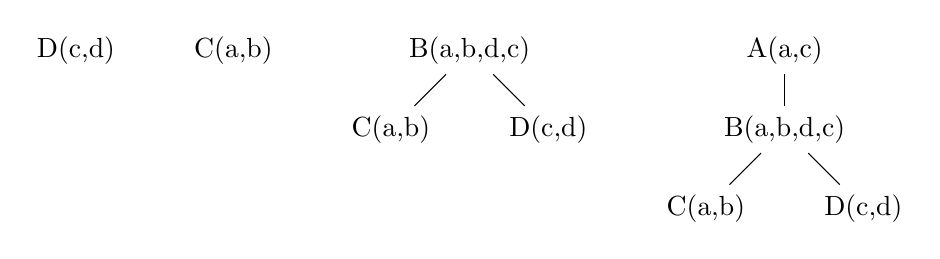
\begin{tikzpicture}
        \node (D1) at (0,0) {D(c,d)};

        \node (C1) at (2,0) {C(a,b)};

        \node (B1) at (5,0) {B(a,b,d,c)};
        \node (B2) at (4, -1) {C(a,b)};
        \node (B3) at (6, -1) {D(c,d)};
        \draw (B1) -- (B2);
        \draw (B1) -- (B3);

        \node (A1) at (9,0) {A(a,c)};
        \node (A2) at (9,-1) {B(a,b,d,c)};
        \node (A3) at (8, -2) {C(a,b)};
        \node (A4) at (10, -2) {D(c,d)};
        \draw (A1) -- (A2);
        \draw (A2) -- (A3);
        \draw (A2) -- (A4);
    \end{tikzpicture}

    The proof tree for $A(b,d)$ already contains proofs for all the other elements of the program so it would be enough to check this single tree.
\end{example}

If we want to check a complete datalog result, we therefore do not have to include a proof tree for every element as they can occur in other proof trees already. We formalize this using the element member function that is true if this element is the root or a member in a subtree.

\begin{lstlisting}
def (.\elementMember.) (a: A) (t: tree A): Bool  :=
    match t with
    | tree.node a' l => (a=a') ∨
        List.any l.attach (fun ⟨x, _h⟩ => elementMember a x)
\end{lstlisting}

A tree is valid if all subtrees are valid. In the rule case, we explicitly required this, whereas there are no subtrees in the database case. Any element member is the root of some subtree and therefore any element member of a valid proof tree is in the proof-theoretic semantics 

(\allTreeElementsOfValidTreeInSemantics).

This allows us to establish the alternative property of validateTreeList. We added the requirement of all proofs being valid to prove the back direction. As the validity of a proof tree is in general not preserved under permutation, it is not sufficient to just require every element member to be in the proof-theoretic semantics.

\begin{lemma}[\validateTreeListUnitIffSubsetSemanticsAndAllElementsHaveValidTrees]
    Let $P$ be a program, $d$ be a database and $l$ a list of proof trees. Then validateTreeList returns ok iff all element members of the trees in $l$ are in the proof-theoretic semantics and all trees in $l$ are valid.
\end{lemma}
\begin{proof}
    For the forward direction, we already noted that if validateTreeList returns ok, then every tree in $l$ must be valid. By the previous lemma therefore any element member of one of these trees is in the proof-theoretic semantics.

    For the back-direction follows from the previous observation, that validateTreeList returns ok iff all trees in $l$ are valid.
\end{proof}

Now it is enough to pass just the proof tree for $A(a,c)$ from our example into the checker to validate the whole input and use in general fewer trees. 
